\begin{frame}{Categorization of cryptographic primitives}
Cryptographic primitives are the tools that can be used to achieve \textit{confidentiality}, \textit{integrity}, \textit{authentication}, and \textit{non-repudiation}.
    \begin{figure}
        \centering
        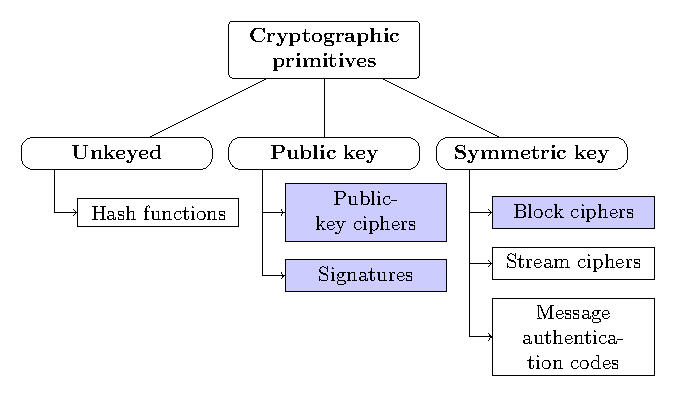
\includegraphics[width=0.7\textwidth]{fig/primitives.pdf}
        \caption{Categorization of cryptographic primitives. The ones highlighted in blue color will be discussed in this course.}
    \end{figure}
\end{frame}

\begin{frame}{Insecure communication}
    \begin{itemize}
        \item We have mentioned three types of ciphers: public-key ciphers, block ciphers, and stream ciphers.
        \item Ciphers are also called cryptosystems.
        \item When we use ciphers, we normally assume insecure communication.
        \item A popular example setting is that Alice would like to send messages to Bob but Eve is also listening to the communication.
    \end{itemize}
\end{frame}

\begin{frame}{Physical attacks on cryptographic primitives}
We will be focusing on physical attacks on
    \begin{itemize}
        \item Symmetric block ciphers 
        \item Public key ciphers
    \end{itemize}
Physical attacks also apply to other cryptographic primitives
\begin{itemize}
    \item Hemme, Ludger, and Lars Hoffmann. ``Differential fault analysis on the SHA1 compression function.'' 2011 Workshop on Fault Diagnosis and Tolerance in Cryptography. IEEE, 2011.
    \item Hao, Ronglin, et al. ``Algebraic fault attack on the SHA-256 compression function.'' International Journal of Research in Computer Science 4.2 (2014): 1-9.
    \item Kahri, Fatma, et al. ``Fault Attacks Resistant Architecture for KECCAK Hash Function.'' Journal of Advanced Computer Science and Applications 5.8 (2017): 237-243.
    \item $\dots$
\end{itemize}
\end{frame}

\begin{frame}{Insecure communication channel}
%%Alice
\begin{tikzpicture}[remember picture,overlay]
     \node[xshift=-13cm,yshift=4.5cm] at (current page.south east)
    {Alice};
    \node[xshift=-13cm,yshift=2.5cm] at (current page.south east) {
\includegraphics[width = 0.15\textwidth]{fig/Alice.png}};
    \node[xshift=-13cm,yshift=0.3cm] at (current page.south east)
    {\picsrc{https://www.pngwing.com/en/free-png-zhbsy}
    };
\end{tikzpicture}
%%Bob
\begin{tikzpicture}[remember picture,overlay]
     \node[xshift=-3cm,yshift=4.5cm] at (current page.south east)
    {Bob};
    \node[xshift=-3cm,yshift=2.5cm] at (current page.south east) {
\includegraphics[width = 0.13\textwidth]{fig/Bob.png}};
    \node[xshift=-3cm,yshift=0.3cm] at (current page.south east)
    {\picsrc{https://alicebobstory.com/}};
\end{tikzpicture}
%%Eve
\begin{tikzpicture}[remember picture,overlay]
    \node[xshift=-8cm,yshift=6cm] at (current page.south east) {
\includegraphics[width = 0.25\textwidth]{fig/Eve.jpg}};
    \node[xshift=-8cm,yshift=7.8cm] at (current page.south east)
    {Eve};
    \node[xshift=-8cm,yshift=4cm] at (current page.south east)
    {\picsrc{https://pngtree.com/}};
\end{tikzpicture}
\end{frame}

\begin{frame}{Encryption and decryption}
    \begin{itemize}
        \item When we use ciphers, we normally assume insecure communication.
        \item A popular example setting is that Alice would like to send messages to Bob but Eve is also listening to the communication.
       \item The goal of Alice is to make sure that even if Eve can intercept what was sent, she will not be able to find the original message.
       \item To do so, Alice will first \textit{encrypt} the message, or the \textit{plaintext}, and send the \textit{ciphertext} to Bob, instead of the original message.
      \item Bob will then \textit{decrypt} the ciphertext to get the plaintext.
      \item For this communication to work, there must be a \textit{key} for encryption and decryption.
     \item It is clear that the decryption key should be secret from Eve
     \item Also, a basic requirement is that the algorithm for \textit{encryption/decryption} should be designed in a way that Eve cannot easily brute force the plaintext with the knowledge of the ciphertext.
    \end{itemize}
\end{frame}

\begin{frame}{Cryptosystem}
\begin{definition}
A \textit{cryptosystem} is a tuple $(\mathcal{P},\mathcal{C},\mathcal{K},\mathcal{E},\mathcal{D})$ with the following properties.
\begin{itemize}
        \item $\mathcal{P}$ is a finite set of plaintexts, called \textit{plaintext space}.
        \item $\mathcal{C}$ is a finite set of ciphertexts, called \textit{ciphertext space}.
        \item $\mathcal{K}$ is a finite set of keys, called \textit{key space}.
        \item $\mathcal{E}=\Set{E_k:k\in\mathcal{K}}$, where $E_k:\mathcal{P}\to\mathcal{C}$ is an \textit{encryption function}.
        \item $\mathcal{D}=\Set{D_k:k\in\mathcal{K}}$, where $D_k:\mathcal{C}\to\mathcal{P}$ is a \textit{decryption function}.
        \item For each $e\in\mathcal{K}$, there exists $d\in\mathcal{K}$ such that $D_d(E_e(p))=p$ for all $p\in\mathcal{P}$.
\end{itemize}
If $e=d$, the cryptosystem is called a \textit{symmetric key cryptosystem}.
Otherwise, it is called a \textit{public-key/asymmetric cryptosystem}.
\end{definition}
\begin{itemize}
    \item There are mainly two types of symmetric ciphers: \textit{block ciphers} and \textit{stream ciphers}.
\end{itemize}
\end{frame}

\begin{frame}{Block ciphers}
\begin{definition}[Block cipher]
A \textit{block cipher} is a symmetric key cryptosystem with $\mathcal{P}=\mathcal{C}=\mathcal{A}^n$ for some alphabet $\mathcal{A}$ and positive integer $n$.
$n$ is called the \textit{block length}.
\end{definition}
\begin{itemize}
    \item For classical ciphers that we will see in this video, $\mathcal{A}=\ZZ_{26}$.
    \item For modern cryptosystems that we will discuss in the next video, $\mathcal{A}=\FF_2=\Set{0,1}$.
\end{itemize}
\end{frame}

\begin{frame}{Converting message to plaintext}
    \begin{itemize}
        \item An important aspect to clarify is how the message that Alice intends to send is represented as plaintext.
        \item For classical ciphers, which we will discuss in a while, we will only consider messages consisting of English letters (\texttt{A} -- \texttt{Z}), and we map each letter to an element in $\ZZ_{26}$ - the set of remainders when dividing an integer by $26$
        \item The plaintext spaces are vector spaces over $\ZZ_{26}$.
    \end{itemize}
\begin{table}
\centering
\begin{tabular}{cccccccccccccccccccccccccc}
\begin{tabular}{cccccccccccccccccccc}
\texttt{A} & \texttt{B} & \texttt{C} & \texttt{D} & \texttt{E} & \texttt{F} & \texttt{G} & \texttt{H} & \texttt{I} & \texttt{J} & \texttt{K}  & \texttt{L}  & \texttt{M}  & \texttt{N}  & \texttt{O}  & \texttt{P}  & \texttt{Q}  & \texttt{R}  & \texttt{S}  & \texttt{T}   \\
0 & 1 & 2 & 3 & 4 & 5 & 6 & 7 & 8 & 9 & 10 & 11 & 12 & 13 & 14 & 15 & 16 & 17 & 18 & 19 
\end{tabular}\\
\begin{tabular}{cccccc}
 \texttt{U}  & \texttt{V}  & \texttt{W}  & \texttt{X}  & \texttt{Y}  & \texttt{Z} \\
20 & 21 & 22 & 23 & 24 & 25
\end{tabular}
\end{tabular}
\caption{Converting English letters to elements in $\ZZ_{26}$.}
\end{table}
\end{frame}

\begin{frame}{Converting message to plaintext -- modern cipher}
    \begin{itemize}
        \item In modern computers, we store data in binary digits (bits).
        \item An $8-$bit binary string is called a byte 
        \item Computers often operate on a few bytes at a time.
        \item For example, a 64-bit processor operates on eight bytes at a time.
        \item In computer architecture, a \textit{word} is defined as the unit of data of (at most) a certain bit length that can be addressed and moved between storage and the processor.
        \begin{itemize}
            \item For a 64-bit processor, the word length is 64 bits. 
        \end{itemize}
    \end{itemize}
\end{frame}

\begin{frame}{Converting message to plaintext -- modern cipher}
    \begin{itemize}
        \item A byte can be represented as a decimal number between $0$ and $255$ or as a hexadecimal number between \texttt{00}$_{16}$ and \texttt{FF}$_{16}$.
        \item When modern cryptographic algorithms are used, the messages are converted to plaintexts which are $n$-bit binary strings, where $n$ is a multiple of $8$.
\end{itemize}
\begin{table}
\begin{subtable}{0.45\textwidth}
\centering
    \begin{tabular}{|c|c|c|}\hline
               $A$  & 01000001 & \texttt{41}\\
               $B$  & 01000010 & \texttt{42}\\
               $a$  & 01100001 & \texttt{61}\\
               $b$  & 01100010 & \texttt{62}\\
               $?$  & 00111111 & \texttt{3F}\\\hline
    \end{tabular}\quad
    \caption{ASCII}
\end{subtable}
\begin{subtable}{0.45\textwidth}
\centering
    \begin{tabular}{|c|c|c|}\hline
               $\acute{A}$  & 11000001 & \texttt{C1}\\
               $\ddot{A}$  & 11000100 & \texttt{C4}\\
               $\acute{I}$  & 11001101& \texttt{CD}\\
               $\times$  & 11010111 & \texttt{D7}\\
               $\div$  & 11110111 & \texttt{F7}\\\hline
    \end{tabular}
    \caption{UTF-8}
\end{subtable}
\caption{Examples of methods for converting message symbols to bytes.
The second column in each table is the binary representation of the byte value and the third column is the corresponding hexadecimal representation.}
\end{table}
\end{frame}

\begin{frame}{Kerckhoffs' principle}
When the security of a cryptosystem is analyzed, \textit{Kerckhoffs' principle} is always followed.
\begin{definition}[Kerckhoffs' principle]
The security of a cryptosystem should depend only on the secrecy of the key.
\end{definition}
\noindent
In other words, everything is public knowledge except for the secret key.
\end{frame}

\begin{frame}{Computations in $\ZZ_{26}$}
    \begin{itemize}
        \item Addition, subtraction and multiplications are done modulo $26$
        \begin{itemize}
            \item First compute the addition, subtraction or multiplication
            \item Then compute the remainder divided by $26$
        \end{itemize}
        \item Notation: $\mo 26$
    \end{itemize}
    \begin{example}
    \[
    2+6\mo26=8,\quad 20+10\mo26=30\mo26=4,\quad (-2)+7\mo26=5,
    \]
    \[
    2\times6\mo26=12,\quad 20\times10\mo26=200\mo26=18,
    \]
    \[
    (-2)\times7\mo26=-14\mo26=12
    \]
    \end{example}
\end{frame}

\begin{frame}{Shift cipher}
    \begin{definition}[Shift cipher]
Let $\mathcal{P}=\mathcal{C}=\mathcal{K}=\ZZ_{26}$.
For each $k\in\mathcal{K}$, define
    \[
    E_k: \ZZ_{26}\to\ZZ_{26},\quad  p\mapsto p+k \mo 26;
    \quad
    D_k: \ZZ_{26}\to\ZZ_{26},\quad  c\mapsto c-k \mo 26.
    \]
The cryptosystem $(\mathcal{P},\mathcal{C},\mathcal{K},\mathcal{E},\mathcal{D})$, where $\mathcal{E}=\Set{E_k:k\in\mathcal{K}}$, and $\mathcal{D}=\Set{D_k:k\in\mathcal{K}}$, is called the \textit{shift cipher}.
\end{definition}
\begin{alertblock}{Remark}
    It is easy to see that there are only $25$ possible key values and an attacker can break the cipher by trying all possible keys.
\end{alertblock}
\end{frame}

\begin{frame}{Shift cipher -- Example}
\begin{example}
Let $k=5$, 
\[
E_k(\texttt{A})=0+5\mo 26=\texttt{F},\quad E_k(\texttt{Z})=25+5\mo 26=4\mo 26=\texttt{E}.
\]
To encrypt a message, we can use the following table and replace letters in the first row with those in the second row.
\begin{table}
\centering
\begin{tabular}{cccccccccccccccccccc}
\texttt{A} & \texttt{B}& \texttt{C} & \texttt{D} & \texttt{E} & \texttt{F}  & \texttt{G} & \texttt{H} & \texttt{I} & \texttt{J} & \texttt{K}  & \texttt{L}  & \texttt{M}  & \texttt{N}  & \texttt{O}  & \texttt{P}  & \texttt{Q}   & \texttt{R}  & \texttt{S}  & \texttt{T}   \\
\texttt{F}  & \texttt{G} & \texttt{H} & \texttt{I} & \texttt{J} & \texttt{K} & \texttt{L} & \texttt{M} & \texttt{N} & \texttt{O} & \texttt{P} & \texttt{Q}  & \texttt{R} & \texttt{S} & \texttt{T} & \texttt{U} & \texttt{V} & \texttt{W} & \texttt{X} & \texttt{Y} 
\end{tabular}\\\vspace{0.3cm}
\begin{tabular}{cccccc}
 \texttt{U}  & \texttt{V}  & \texttt{W}  & \texttt{X}  & \texttt{Y}  & \texttt{Z}  \\
\texttt{Z} & \texttt{A} & \texttt{B}& \texttt{C} & \texttt{D} & \texttt{E}
\end{tabular}
\end{table}
Suppose the message is 
\[
\texttt{I LOVE CRYPTOGRAPHY}
\]
Then the corresponding ciphertext (omitting the white spaces) is ?
\end{example}
\end{frame}

\begin{frame}{Shift cipher}
We note that encrypting using a key $k$ is the same as shifting the letters by $k$ positions, hence the name ``shift cipher''.
\begin{example}
Let $k=5$, 
To encrypt a message, we can use the following table and replace letters in the first row with those in the second row.
\begin{table}
\centering
\begin{tabular}{cccccccccccccccccccc}
\texttt{A} & \texttt{B}& \texttt{C} & \texttt{D} & \texttt{E} & \texttt{F}  & \texttt{G} & \texttt{H} & \texttt{I} & \texttt{J} & \texttt{K}  & \texttt{L}  & \texttt{M}  & \texttt{N}  & \texttt{O}  & \texttt{P}  & \texttt{Q}   & \texttt{R}  & \texttt{S}  & \texttt{T}   \\
\texttt{F}  & \texttt{G} & \texttt{H} & \texttt{I} & \texttt{J} & \texttt{K} & \texttt{L} & \texttt{M} & \texttt{N} & \texttt{O} & \texttt{P} & \texttt{Q}  & \texttt{R} & \texttt{S} & \texttt{T} & \texttt{U} & \texttt{V} & \texttt{W} & \texttt{X} & \texttt{Y} 
\end{tabular}\\\vspace{0.3cm}
\begin{tabular}{cccccc}
 \texttt{U}  & \texttt{V}  & \texttt{W}  & \texttt{X}  & \texttt{Y}  & \texttt{Z}  \\
\texttt{Z} & \texttt{A} & \texttt{B}& \texttt{C} & \texttt{D} & \texttt{E}
\end{tabular}
\end{table}
Suppose the message is 
\[
\texttt{I LOVE CRYPTOGRAPHY}
\]
Then the corresponding ciphertext (omitting the white spaces) is 
\[
\texttt{NQTAJHWDUYTLWFUMD}.
\]
\end{example}
\end{frame}
